\documentclass{beamer}

\mode<presentation>
{
  \usetheme{Warsaw}      % or try Darmstadt, Madrid, Warsaw, ...
  \usecolortheme{rose} % or try albatross, beaver, crane, ...
  \usefonttheme{default}  % or try serif, structurebold, ...
  \setbeamertemplate{navigation symbols}{}
  \setbeamertemplate{caption}[numbered]
} 

\usepackage[english]{babel}
\usepackage[utf8x]{inputenc}
\usepackage{amsthm,amsmath,amssymb}
\usepackage{geometry}
\usepackage{float}
\usepackage{graphicx}
\usepackage{tikz}
\usepackage{url}

\title{Parallel FFT for PDEs and parallel in time}
\author{Frederick Law, Evan Toler, and Scott Weady}
% \institute{Courant Institute}
\date{May 4, 2020}

\begin{document}

\begin{frame} %%%%%%%%%%%%%%%%%%%%%%%%%%%%%%%%%%%%%%%%
  \titlepage
\end{frame}



\begin{frame}{Problem Summary} %%%%%%%%%%%%%%%%%%%%%%%%%%%%%%%%%%%%%%%%

\begin{itemize}
  \item Solving the Korteweg–de Vries (KdV) equation, a nonlinear PDE: 
  $u_t = -u_{xxx} + 3(u^2)_x$
  \pause
  \item Using a pseudospectral approach. For the $k$th Fourier mode
  \begin{equation*}
  \widehat u_t = -(ik)^3\widehat u 
    + 3ik \mathcal (F[(\mathcal F^{-1}[\widehat u])^2])_k
  \end{equation*}
  \pause
  \item Two sources of parallelism
  \begin{itemize}
      \item A parallel FFT algorithm for the operators $\mathcal F$ and $\mathcal F^{-1}$
      \item A solver for the system of ODEs in Fourier space: Parareal\footnote{Images 
      from \url{https://en.wikipedia.org/wiki/Parareal}}
  \end{itemize}
\end{itemize}

\begin{figure}[hb]
    \centering
    % 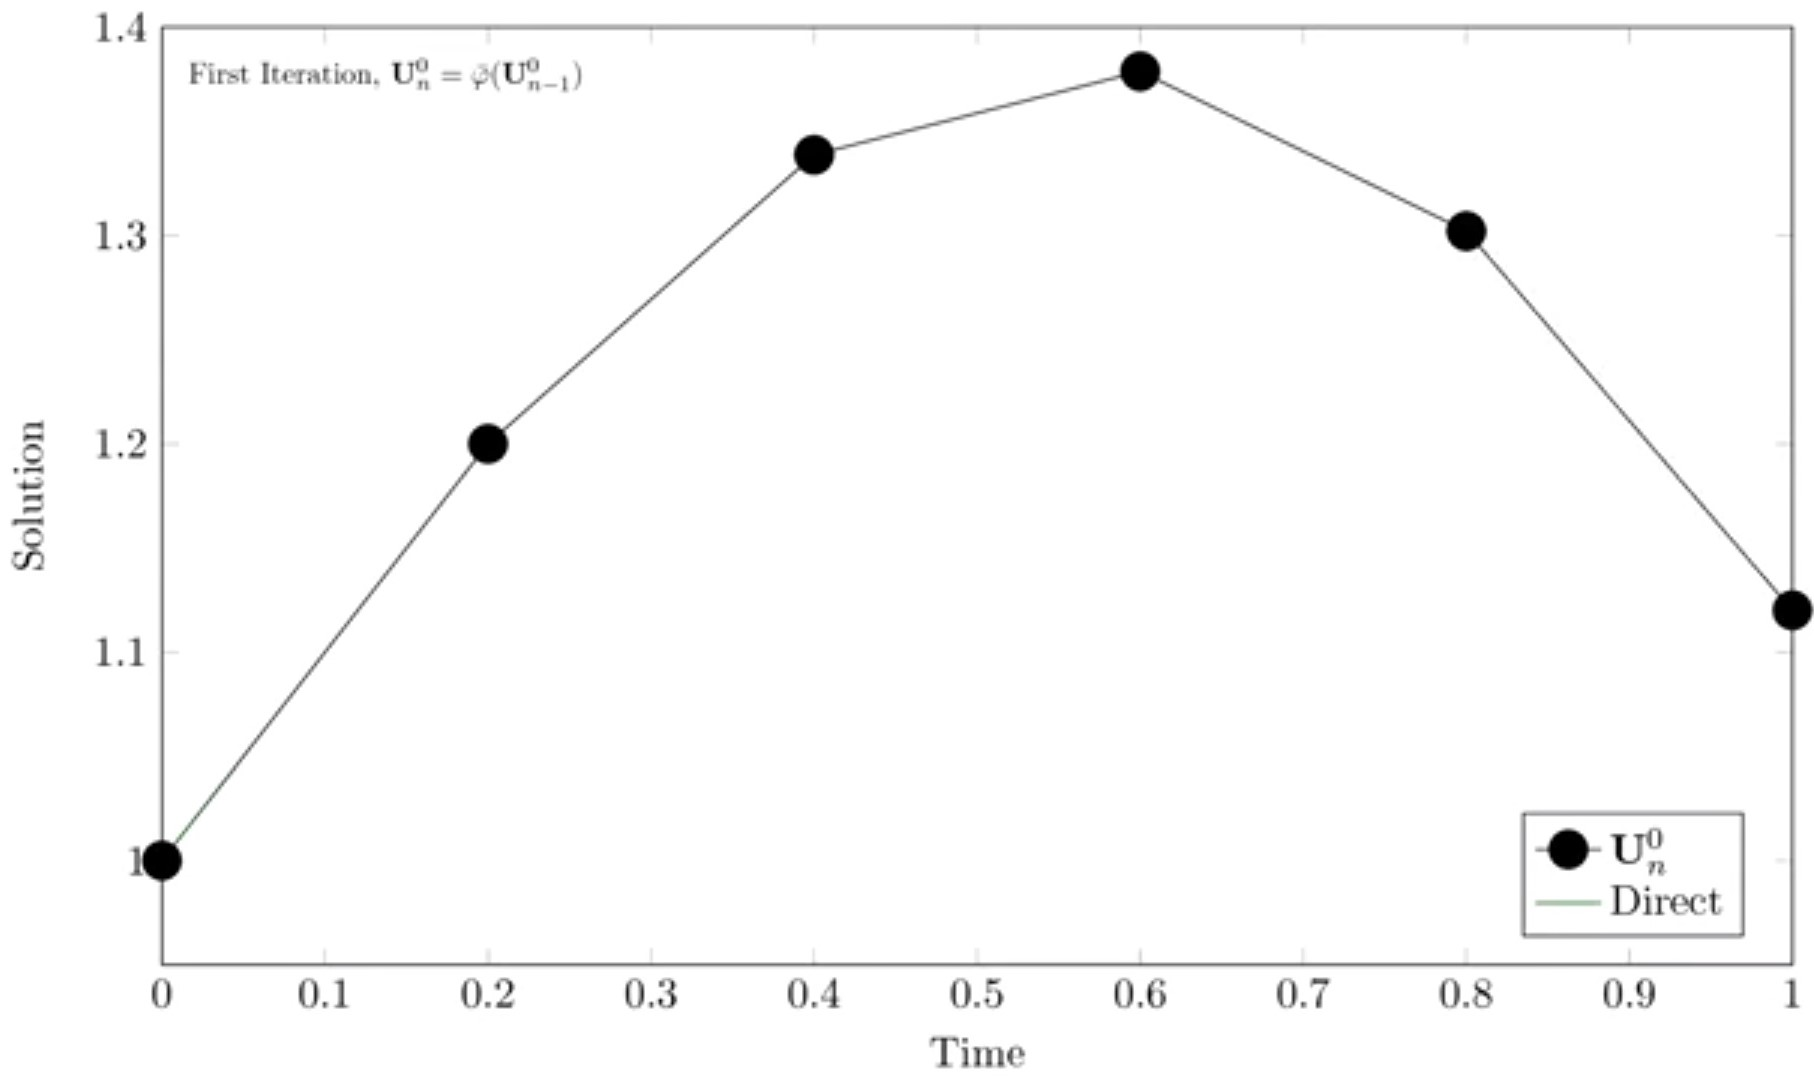
\includegraphics[width=0.45\textwidth]{Images/parareal1.jpg}
    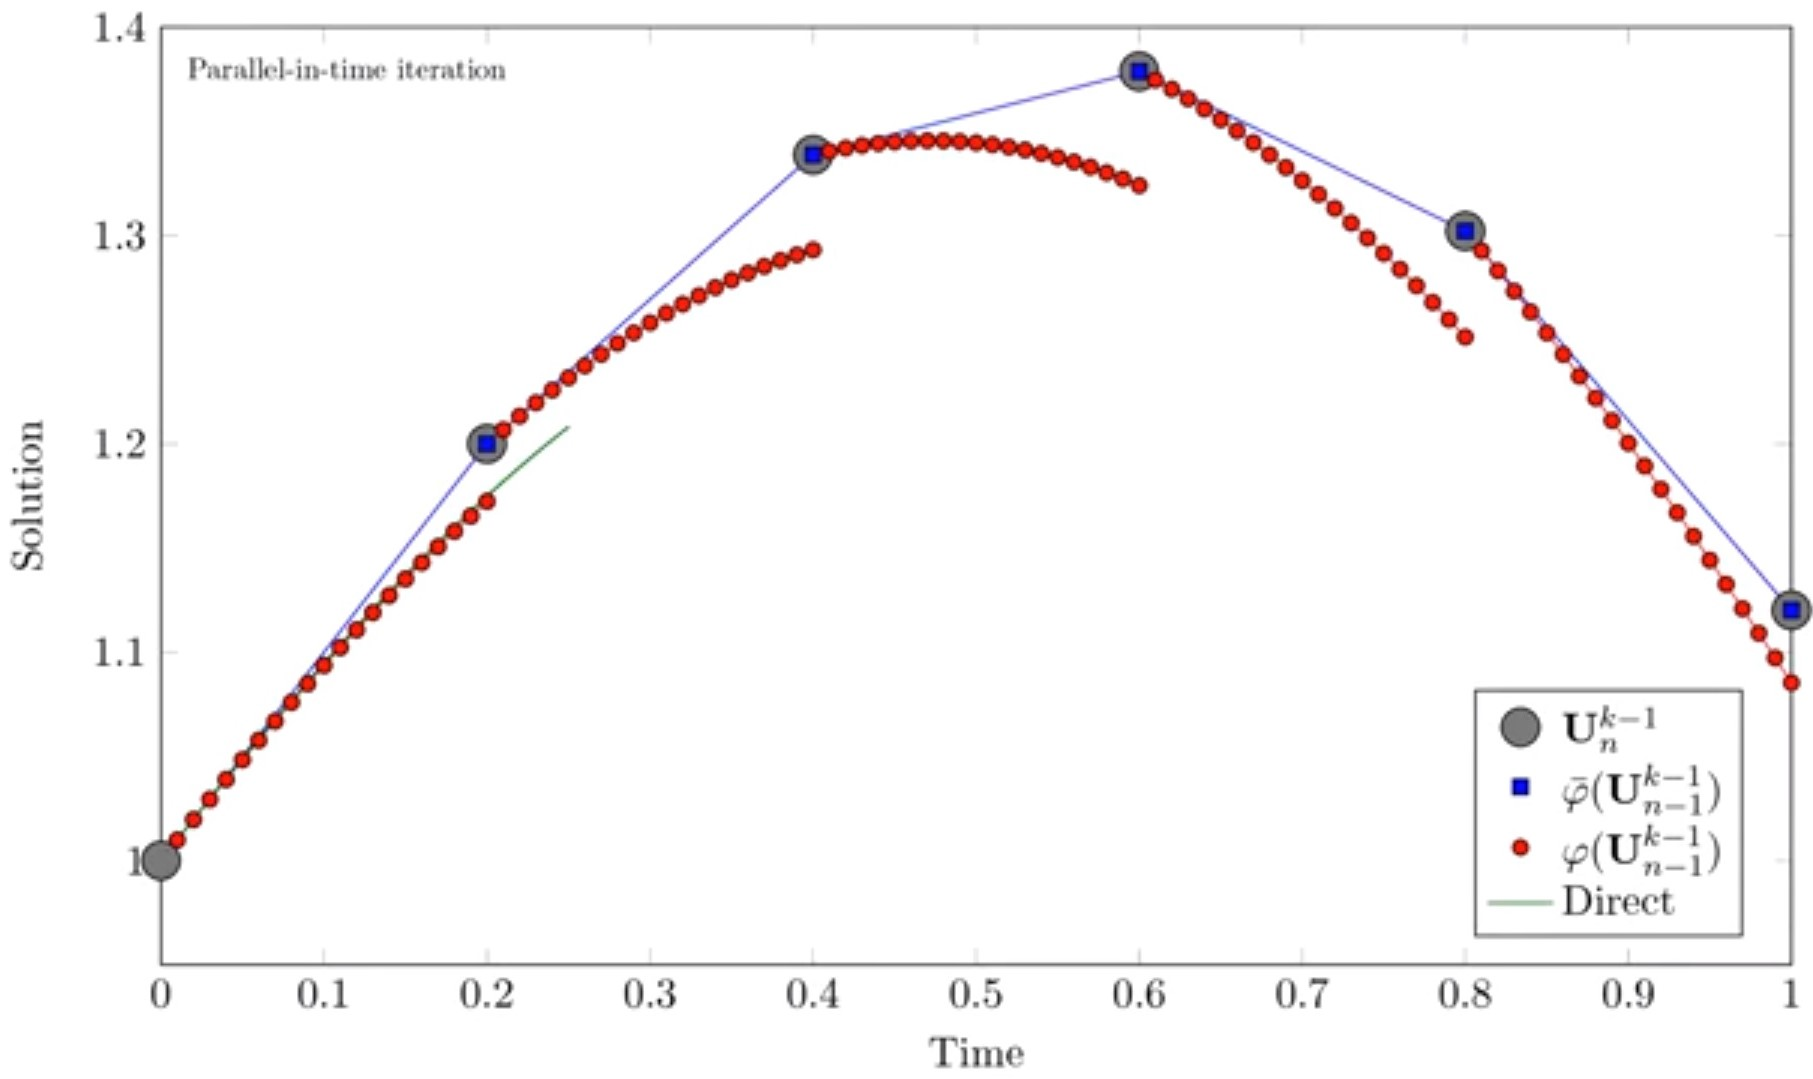
\includegraphics[scale=0.1]{Images/parareal2.jpg}
    \pause
    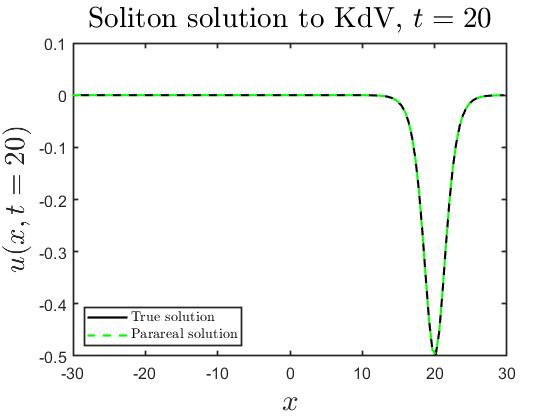
\includegraphics[scale=0.2]{Images/kdv_sol.jpg}
    % 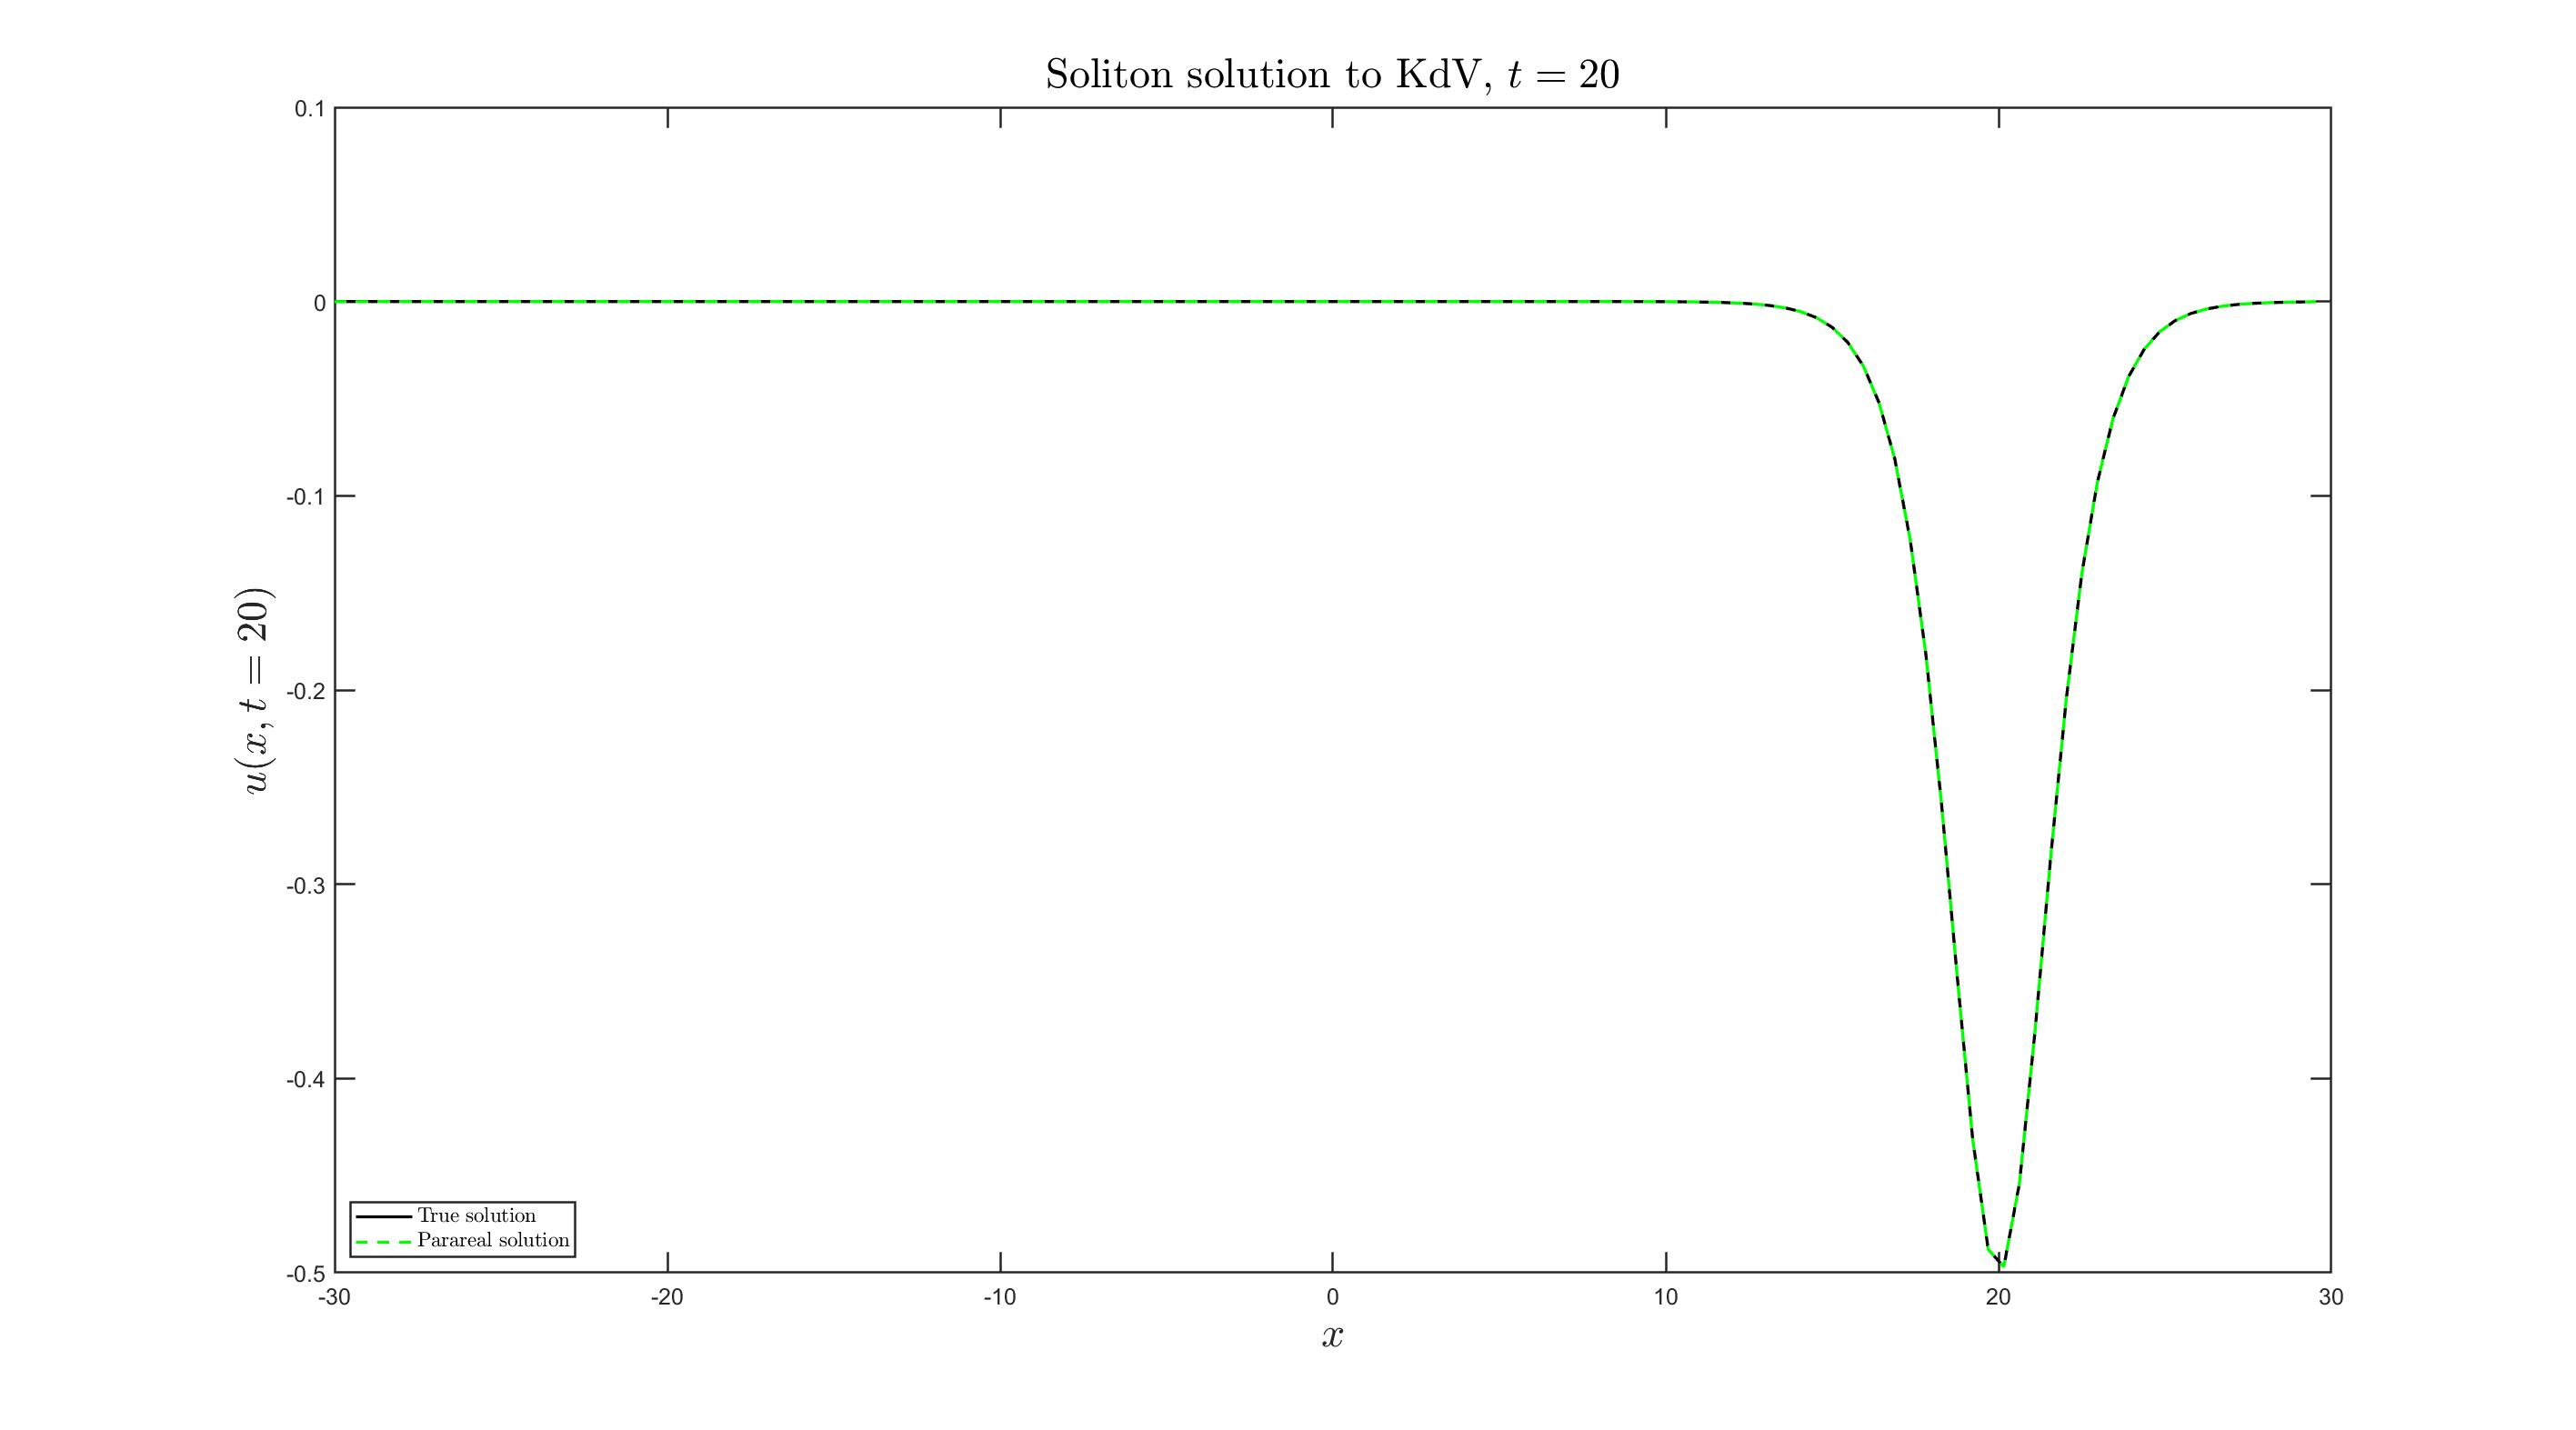
\includegraphics[scale=0.05]{Images/kdv_sol2.jpg}
    % \caption{An illustration of Parareal for an example ODE}
    % 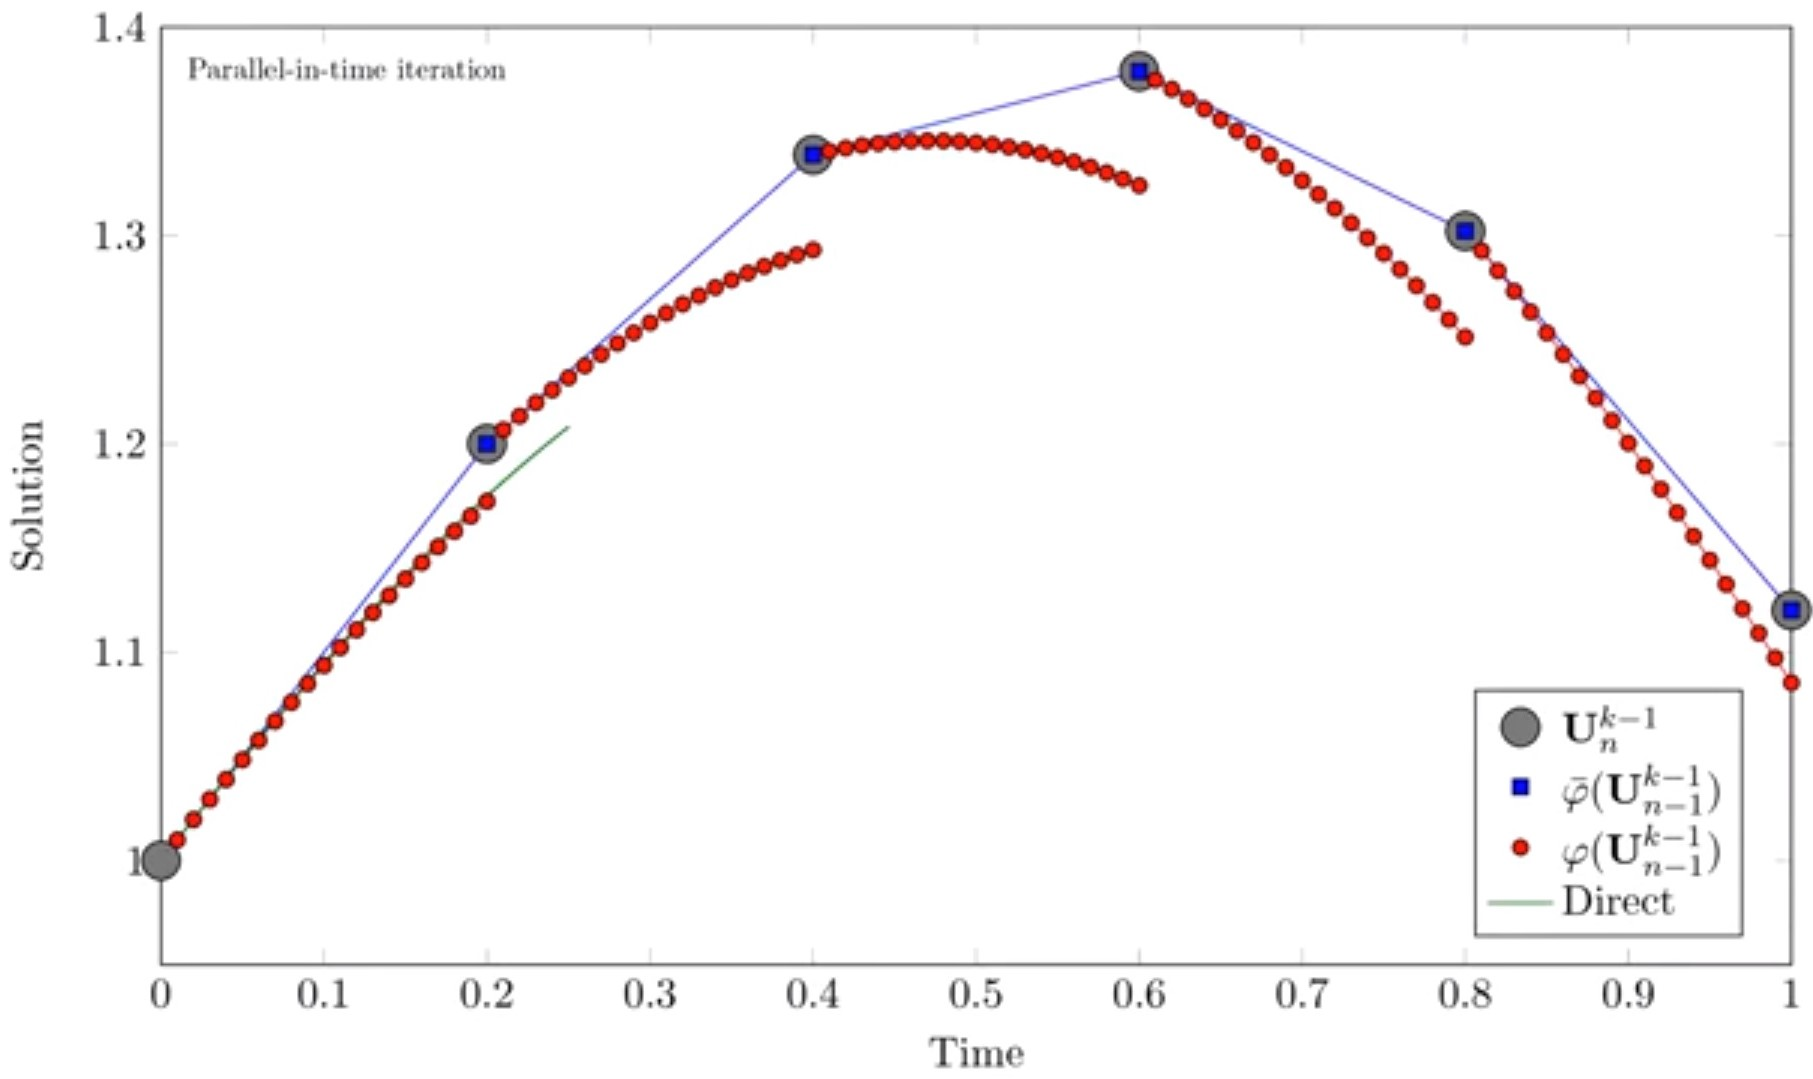
\includegraphics[width=.45\textwidth]{Images/parareal2.jpg}
    % 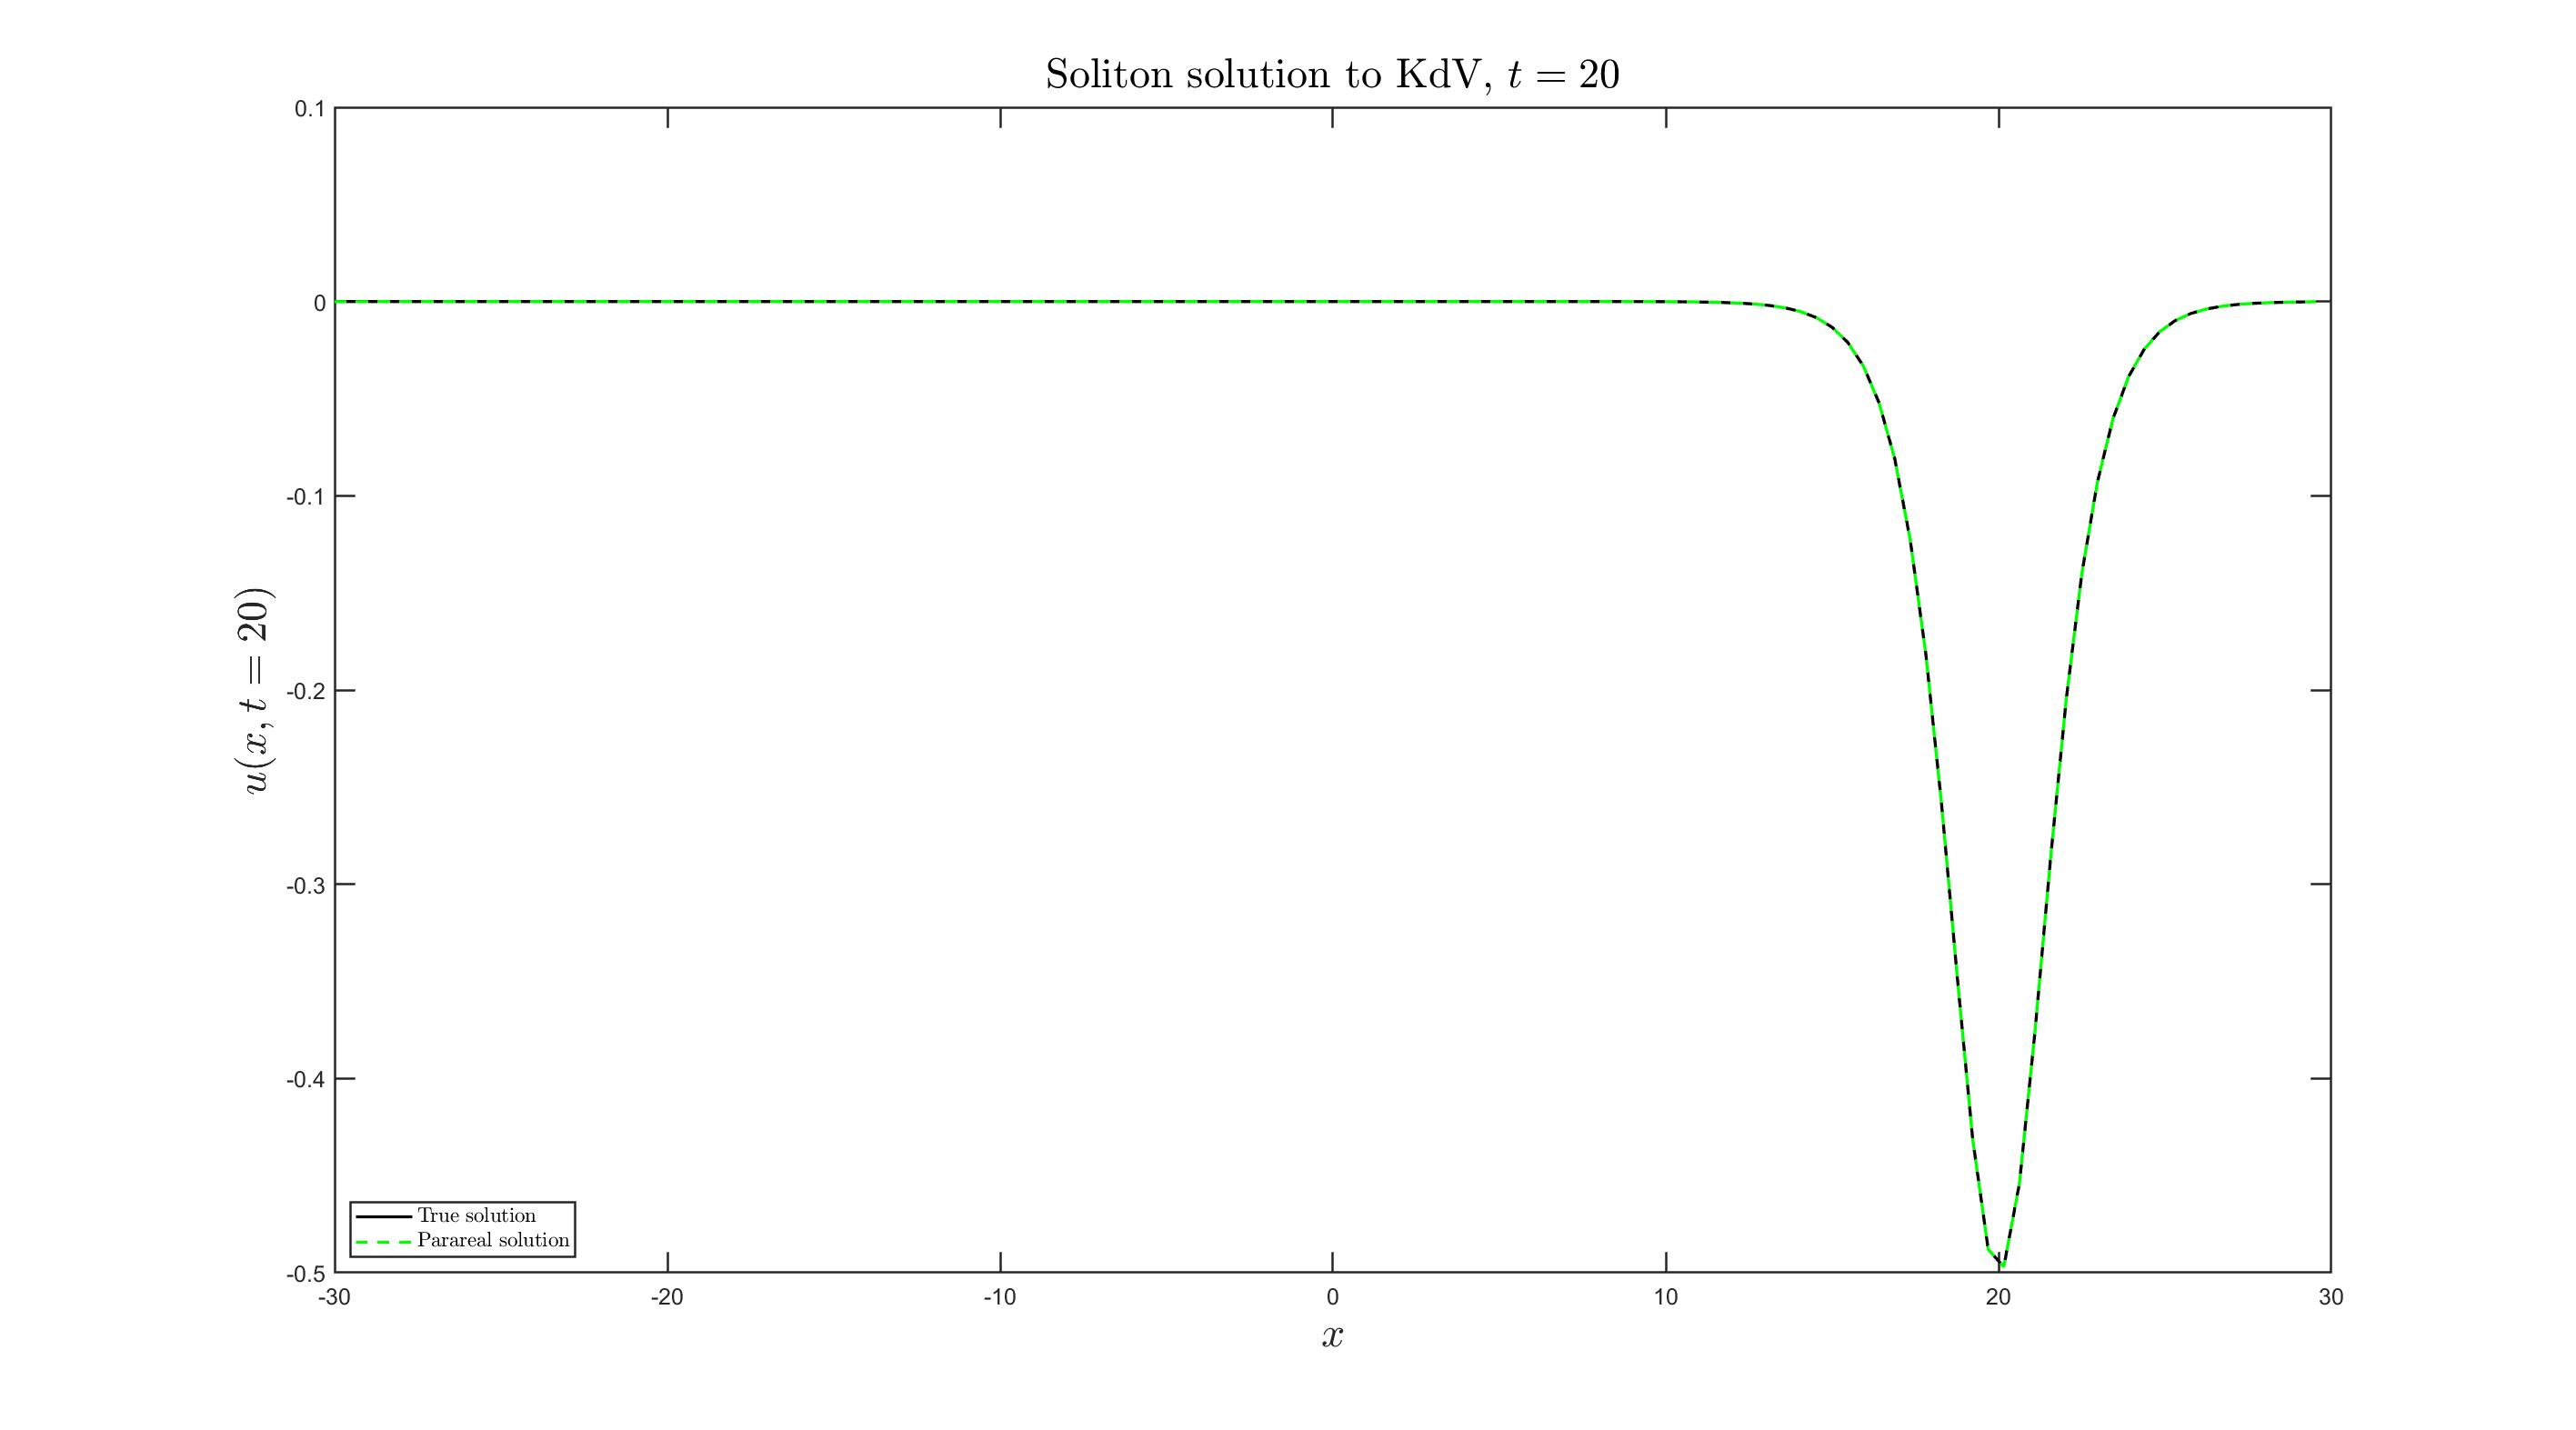
\includegraphics[width=.45\textwidth]{Images/kdv_sol2.jpg}
    \label{fig:parareal}
\end{figure}

\end{frame}


\begin{frame}{Thread Management} %%%%%%%%%%%%%%%%%%%%%%%%%%%%%%%%%%%%%%%%

\begin{itemize}
  \item We used OpenMP to implement Parareal and the FFT
  \begin{itemize}
      \item FFT: hierarchy of \texttt{task}s with the Cooley-Tukey recursive approach
      \begin{itemize}
          \item Repeat the iteration $\text{FFT}(u) = \text{FFT}(u_{\text{even}}) 
          + \text{FFT}(u_{\text{odd}})$
          \item Optimal to assign $2^p$ threads for the FFT for some $p$.
      \end{itemize}
      \item Parareal: parallel \texttt{for} loops over each time interval
      \begin{itemize}
          \item Each thread in Parareal spawns threads to perform FFTs.
      \end{itemize}
  \end{itemize}
  
  \pause
  
  \item Performance holding all other parameters constant:
\end{itemize}

% ./parareal-kdv 256 .01 100 10
% changing thread count macros
\begin{table}[h!]
    \centering
    \begin{tabular}{|c|c|c|}
    \hline
    Parareal threads & FFT threads & Runtime (s) \\
    \hline\hline
    32 & 2 & 1.1650 \\
    16 & 4 & 1.2019 \\
    8 & 8  & 1.4830 \\
    4 & 16 & 1.9339 \\
    \hline
    \end{tabular}
    \caption{Performance for different thread distributions,
    with a fixed number of total threads. Using 256 Fourier modes
    to integrate from $t=0$ to $t=0.1$.}
    \label{tab:thread_dist}
\end{table}
\end{frame}


\begin{frame}{Performance and Speedup} %%%%%%%%%%%%%%%%%%%%%%%%%%%%%%%%%%%%%%%%

\begin{itemize}
    \item How does the parallel FFT scale in the absence of ODE solvers?
    \item How does Parareal scale for a serial FFT?
    \begin{itemize}
        \item Integrated\footnote{Computations were run on NYU's crunchy5 server.} 
        from time $t=0$ to $t=0.64$
    \end{itemize}
\end{itemize}
\pause

% FFT
% ./fft 1048576 depth (this is 2^20, changing the depth) 
% Parareal
% ./parareal-kdv 128 .01 10 2
% changing thread count macros

\begin{minipage}{0.49\textwidth}
% \begin{table}[h!]
%     \centering
%     \begin{tabular}{|c|c|c|}
%     \hline
%     Threads & Time (s) & Speedup \\
%     \hline\hline
%     1 & 0.83736 & -- \\
%     2 & 0.44884 &  \\
%     4 & 0.27570 &  \\
%     8 & 0.27249 &  \\
%     16 & 0.18154 & \\
%     32 & 0.16772 & \\
%     64 & 0.16376 &
%     \hline
%     \end{tabular}
%     \caption{FFT Scaling. Run with $2^{14}$ Fourier modes.}
%     \label{tab:FFT_scaling}
% \end{table}
\begin{figure}
    \centering
    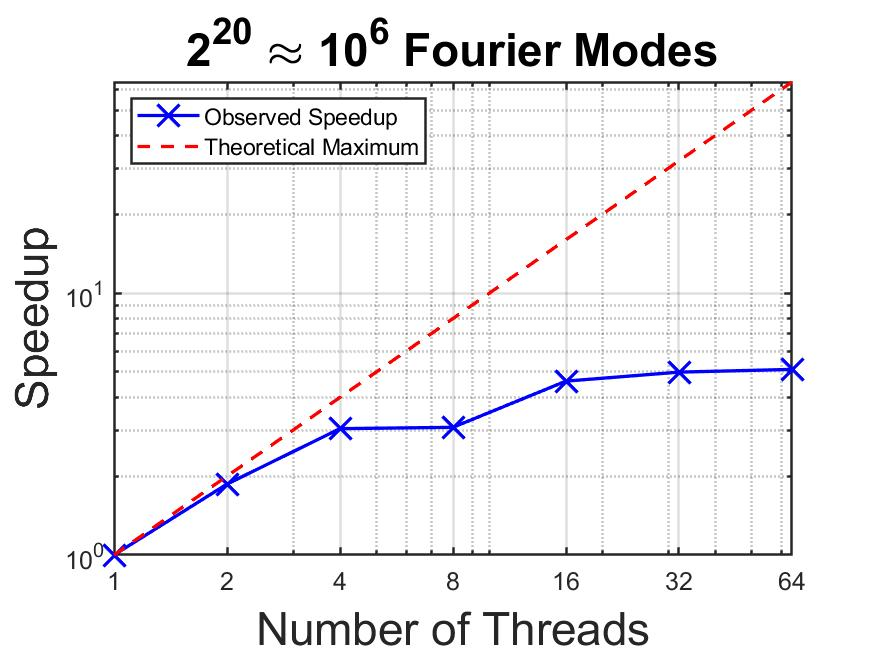
\includegraphics[width=\textwidth]{Images/FFT_scaling.jpg}
    \caption{FFT Scaling}
    \label{fig:FFT_scaling}
\end{figure}
\end{minipage}
\begin{minipage}{0.49\textwidth}
% \begin{table}[h!]
%     \centering
%     \begin{tabular}{|c|c|c|}
%     \hline
%     Threads & Time (s) & Efficiency \\
%     \hline\hline
%     1 & 2.3071 & 0.979611 \\
%     2 & 2.0114 & 0.524040 \\
%     4 & 1.1700 & 0.426221 \\
%     8 & 0.84837 & 0.337112 \\
%     16 & 0.71070 & 0.221393 \\
%     32 & 0.46228 & 0.151590 \\
%     64 & 0.41227 & 0.084713
%     \hline
%     \end{tabular}
%     \caption{Parareal Scaling. Run with $2^8$ Fourier modes.}
%     \label{tab:FFT_scaling}
% \end{table}
\begin{figure}
    \centering
    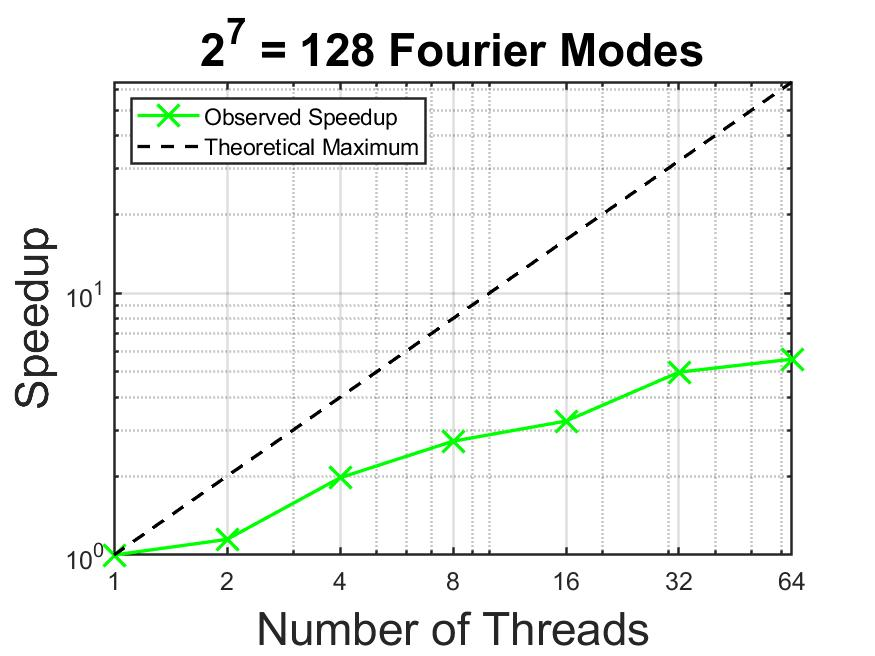
\includegraphics[width=\textwidth]{Images/Parareal_scaling.jpg}
    \caption{Parareal Scaling}
    \label{fig:Parareal_scaling}
\end{figure}
\end{minipage}

\begin{itemize}
    \item \url{https://github.com/fredglaw/HPC-final-project.git}
\end{itemize}

\end{frame}


\end{document}
